\level{2}{Test di integrazione}
	Nella presente sezione vengono riportati i test di integrazione, ovvero quei test che servono per verificare il corretto funzionamento di più moduli assemblati insieme. Per una descrizione completa della sintassi utilizzata nella descrizione di tali test si consulti il documento \insdoc{Norme di Progetto v3.00}. \\
	Questi test sono stati pensati seguendo una strategia \textit{bottom-up}, ossia basata sulla logica di realizzare il prodotto finale a partire dalle singole componenti necessarie per realizzare le funzioni richieste.
	\begin{figure}[H]
		\centering
		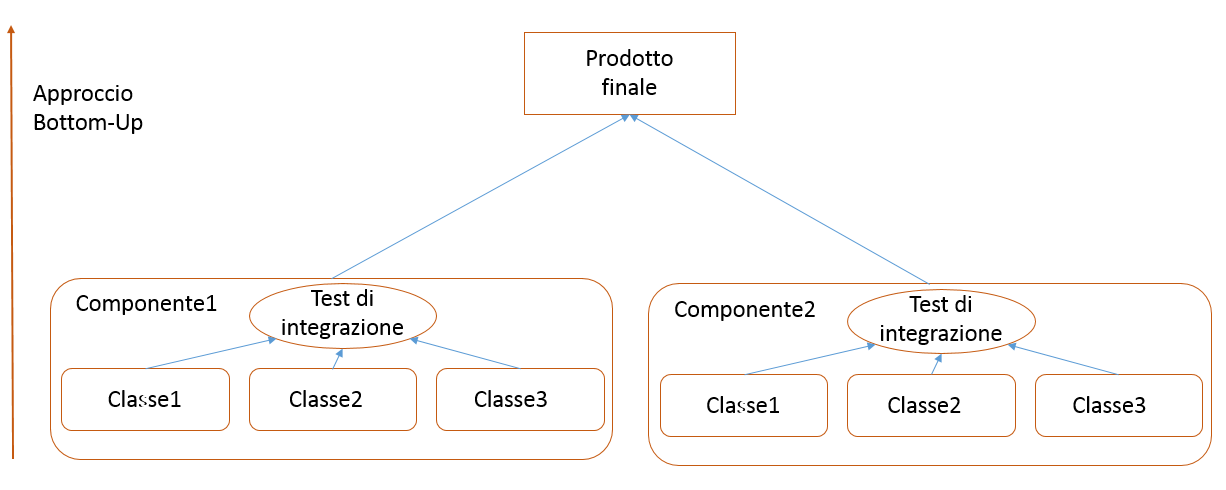
\includegraphics[scale=0.4]{PianoDiQualifica/Pics/bottom-up.png}
		\caption{Modello bottom-up}
	\end{figure}

\begin{longtabu}{| X | X | X[0.9] | X[0.3] |}

			\hline
			\rowfont{\bf}
			Test &
			Descrizione &
			Componenti/Classi &
			Esito \\
			\hline \endhead


%\insglo{Norris}


	TINorris
	&
Test di integrazione finale tra le componenti DataModel, InternalAPIManager e ExternalAPIManager per verificare il comportamento del sistema nel suo complesso.
& \parbox[t]{0.6\textwidth}{
\insglo{Norris}::DataModel\\
\insglo{Norris}::InternalAPI-\\Manager\\
\insglo{Norris}::ExternalAPI-\\Manager}
			& N.I.
			\\ \hline



	TINorrisDataModel
	&
Comportamento del modello: viene verificato che il modello rispetti le aspettative previste, ovvero memorizzi correttamente i dati necessari e li restituisca in un secondo momento senza perdite di informazioni o dati scorretti.
& \parbox[t]{0.6\textwidth}{
\insglo{Norris}::DataModel-\\::NorrisImpl\\
\insglo{Norris}::DataModel-\\::ChartImpl\\
\insglo{Norris}::DataModel-\\::PageImpl}
			& N.I.
			\\ \hline



	TINorrisChartImpl
	&
Comportamento del modello di chart: viene verificato che il modello dei chart memorizzi correttamente le informazioni in base al tipo specifico del chart rappresentato.
& \parbox[t]{0.6\textwidth}{
\insglo{Norris}::DataModel-\\::ChartImpl\\
\insglo{Norris}::DataModel-\\::BarChartImpl\\
\insglo{Norris}::DataModel-\\::LineChartImpl\\
\insglo{Norris}::DataModel-\\::MapChartImpl\\
\insglo{Norris}::DataModel-\\::TableImpl}
			& N.I.
			\\ \hline



	\parbox[t]{0.6\textwidth}{TINorrisInternalAPI-\\Manager}
	&
Funzionamento delle \insglo{API} interne: viene verificato che le \insglo{API} interne apportino al modello le modifiche corrette a seconda dell'azione richiesta.
& \parbox[t]{0.6\textwidth}{
\insglo{Norris}::InternalAPI-\\Manager::InternalAPI-\\Bridge\\
\insglo{Norris}::InternalAPI-\\Manager::ChartBridge\\
\insglo{Norris}::InternalAPI-\\Manager::PageBridge}
			& N.I.
			\\ \hline



	\parbox[t]{0.6\textwidth}{TINorrisExternalAPI-\\Manager}
	&
Funzionamento delle \insglo{API} esterne: viene verificato che le \insglo{API} esterne forniscano le funzione corrette a seconda dei dati rappresentati dal modello.
& \parbox[t]{0.6\textwidth}{
\insglo{Norris}::ExternalAPI-\\Manager::ExternalAPI-\\Controller\\
\insglo{Norris}::ExternalAPI-\\Manager::Authentication-\\Endpoint\\
\insglo{Norris}::ExternalAPI-\\Manager::ListEndpoint\\
\insglo{Norris}::ExternalAPI-\\Manager::ChartEndpoint\\
\insglo{Norris}::ExternalAPI-\\Manager::ChartRef}
			& N.I.
			\\ \hline









%\insglo{Chuck}


	TIChuck
				&
Test di integrazione finale tra tutte le componenti al fine di verificare il sistema nel suo complesso.
			& \parbox[t]{0.6\textwidth}{
\insglo{Chuck}::ChuckManager\\
\insglo{Chuck}::DataModel\\
\insglo{Chuck}::ChartView\\
\insglo{Chuck}::Controller\\
\insglo{Chuck}::Utils}
			& N.I.
			\\ \hline



	TIChuckChuckManager
				&
Comportamento delle \insglo{API} di \insglo{Chuck}: viene verificato che utilizzando l'interfaccia messa a disposizione dallo sviluppatore la componente ChuckManager effettui le operazioni corrette.
			& \parbox[t]{0.6\textwidth}{
\insglo{Chuck}::ChuckManager-\\::ChuckAPIController\\
\insglo{Chuck}::ChuckManager-\\::AuthenticationManager\\
\insglo{Chuck}::ChuckManager-\\::ChartRequester\\
\insglo{Chuck}::ChuckManager-\\::ChartBridge}
			& N.I.
			\\ \hline


	
	\parbox[t]{0.6\textwidth}{TIChuckAuthentication-\\Manager}
				&
Viene verificato che AuthenticationManager effettui l'autenticazione nel modo corretto presso un'istanza valida di \insglo{Norris}.
			& \parbox[t]{0.6\textwidth}{
\insglo{Chuck}::ChuckManager-\\::AuthenticationManager\\
XMLHttpRequest}
			& N.I.
			\\ \hline



	TIChuckChartRequester
				&
Viene verificato che ChartRequester richieda correttamente un grafico presente in un'istanza di \insglo{Norris} e lo mantenga aggiornato.
			& \parbox[t]{0.6\textwidth}{
\insglo{Chuck}::ChuckManager-\\::ChartRequester\\
SocketIOClient}
			& N.I.
			\\ \hline



	TIChuckDataModel
				&
Viene verificato che il modello memorizzi correttamente le informazioni riguardanti i grafici.
			& \parbox[t]{0.6\textwidth}{
\insglo{Chuck}::DataModel-\\::ChuckImpl\\
\insglo{Chuck}::DataModel-\\::ChartImpl}
			& N.I.
			\\ \hline



	TIChuckChartImpl
				&
Viene verificato che il modello dei chart memorizzi correttamente le informazioni in base al tipo specifico del chart rappresentato.
			& \parbox[t]{0.6\textwidth}{
\insglo{Chuck}::DataModel-\\::ChartImpl\\
\insglo{Chuck}::DataModel-\\::BarChartImpl\\
\insglo{Chuck}::DataModel-\\::LineChartImpl\\
\insglo{Chuck}::DataModel-\\::MapChartImpl\\
\insglo{Chuck}::DataModel-\\::TableImpl}
			& N.I.
			\\ \hline



	TIChuckChartView
				&
Viene verificato che la componente ChartView gestisca correttamente la visualizzazione di tutti i tipi di grafici.
			& \parbox[t]{0.6\textwidth}{
\insglo{Chuck}::ChartView-\\::ViewImpl\\
\insglo{Chuck}::ChartView-\\::BarChartView\\
\insglo{Chuck}::ChartView-\\::LineChartView\\
\insglo{Chuck}::ChartView-\\::MapChartView\\
\insglo{Chuck}::ChartView-\\::TableView}
			& N.I.
			\\ \hline



	TIChuckController
				&
Viene verificato che il controller, per tutti i tipi di grafico, gestisca correttamente le notifiche proveniente dalla componente ChartView.
			& \parbox[t]{0.6\textwidth}{
\insglo{Chuck}::Controller-\\::ChartController\\
\insglo{Chuck}::Controller-\\::BarChartController\\
\insglo{Chuck}::Controller-\\::LineChartController\\
\insglo{Chuck}::Controller-\\::MapChartController\\
\insglo{Chuck}::Controller-\\::TableController}
			& N.I.
			\\ \hline



	TIChuckUtils &
Viene verificata la corretta implementazione del \insglo{pattern} Observer.
			& \parbox[t]{0.6\textwidth}{
\insglo{Chuck}::Utils::Observable\\
\insglo{Chuck}::Utils::Observable-\\Impl\\
\insglo{Chuck}::Utils::Observer}
			& N.I.
			\\ \hline









%Applicazione

			TIApplicazione &
			Test di integrazione finale tra le componenti Model, View, Controller
			& \parbox[t]{0.6\textwidth}{
			Applicazione::Model\\
			Applicazione::View\\
			Applicazione::Controller\\
			Applicazione::Utils}
			& N.I.
\\ \hline
			TIApplicazioneModel &
			Viene verificato che il sistema gestisca correttamente la componente Model relativa al \insglo{design pattern} \insglo{MVC}. Più precisamente che memorizzi correttamente i dati relativi ai chart dell'istanza di \insglo{norris} selezionata.
			& \parbox[t]{0.6\textwidth}{
			Applicazione::Model-\\::ChartImpl\\
			Applicazione::Model-\\::BarChartImpl\\
			Applicazione::Model-\\::LineChartImpl\\
			Applicazione::Model-\\::MapChartImpl\\
			Applicazione::Model-\\::TableImpl}
			& N.I.
\\ \hline
			TIApplicazioneView &
			Viene verificato che il sistema gestisca correttamente la componente View del \insglo{pattern} \insglo{MVC}. Più precisamente che gestisca correttamente tutto ciò che concerne la rappresentazione dei chart.
			& \parbox[t]{0.6\textwidth}{
			Applicazione::View-\\::ObservableActivity\\
			Applicazione::View-\\::HomeActivity\\
			Applicazione::View-\\::ListActivity\\
			Applicazione::View-\\::ChartActivity\\
			Applicazione::View-\\::BarChartActivity\\
			Applicazione::View-\\::LineChartActivity\\
			Applicazione::View-\\::MapChartActivity\\
			Applicazione::View-\\::TableActivity}
			& N.I.
\\ \hline
			TIApplicazioneController &
			Viene verificato che il sistema gestisca correttamente la componente Controller del \insglo{design pattern} \insglo{MVC}. Più precisamente viene verificato che il sistema gestisca le azioni dell’utente e che dialoghi in maniera appropriata con il \insglo{server}.
			& \parbox[t]{0.6\textwidth}{
			Applicazione::Controller-\\::Controller\\
			Applicazione::Controller-\\::HomeController\\
			Applicazione::Controller-\\::ListController\\
			Applicazione::Controller-\\::ChartController\\
			Applicazione::Controller-\\::BarChartController\\
			Applicazione::Controller-\\::LineChartController\\
			Applicazione::Controller-\\::MapChartController\\
			Applicazione::Controller-\\::TableController\\
			Applicazione::Controller-\\::JSONParser}
			& N.I.
\\ \hline
			TIApplicazioneUtils &
			Viene verificato che il sistema gestisca correttamente le componenti necessarie per la realizzazione del \insglo{design pattern} Observer.
			& \parbox[t]{0.6\textwidth}{
			Applicazione::Utils\\
			Applicazione::Utils-\\::ObservableImpl}
			& N.I. 
\\ \hline

\caption{Test di integrazione}

\end{longtabu}

	\level{3}*{Tracciamento componenti-test di integrazione}


	\begin{longtabu}{| X | X[0.8] |}

			\hline
			\rowfont{\bf}
			Componenti/Classi	&	Test di integrazione \\ \hline 
			\endhead


			\insglo{Norris} & TINorris \\ \hline 
			\insglo{Norris}::DataModel & TINorrisDataModel \\ \hline 
			\insglo{Norris}::DataModel::ChartImpl & TINorrisChartImpl \\ \hline 
			\insglo{Norris}::InternalAPIManager & TINorrisInternalAPIManager \\ \hline 
			\insglo{Norris}::ExternalAPIManager & TINorrisExternalAPIManager \\ \hline 
			\insglo{Chuck} & TIChuck \\ \hline 
			\insglo{Chuck}::ChuckManager & TIChuckChuckManager \\ \hline 
			\insglo{Chuck}::ChuckManager::AuthenticationManager & TIChuckAuthenticationManager \\ \hline 
			\insglo{Chuck}::ChuckManager::ChartRequester & TIChuckChartRequester \\ \hline 
			\insglo{Chuck}::DataModel & TIChuckDataModel \\ \hline 
			\insglo{Chuck}::DataModel::ChartImpl & TIChuckChartImpl \\ \hline 
			\insglo{Chuck}::ChartView & TIChuckChartView \\ \hline 
			\insglo{Chuck}::Controller & TIChuckController \\ \hline 
			\insglo{Chuck}::Utils & TIChuckUtils \\ \hline 
			Applicazione & TIApplicazione \\ \hline 
			Applicazione::Model & TIApplicazioneModel \\ \hline 
			Applicazione::View & TIApplicazioneView \\ \hline 
			Applicazione::Controller & TIApplicazioneController \\ \hline 
			Applicazione::Utils & TIApplicazioneUtils \\ \hline 




	\caption{Tracciamento componenti - test di integrazione}

\end{longtabu}
